% Chapter 8 -- Least squares and linear regression
\chapter{Least squares and linear regression}\label{ch:lstsq}

More equations than unknowns is not a bug --- it is what real data looks
like. $A\mathbf x=\mathbf b$ almost never has an exact solution once
measurements enter, so we trade ``solve'' for ``fit'': find
$\hat{\mathbf x}$ minimizing $\lVert A\mathbf x-\mathbf b\rVert$. Chapter 5
gives us everything we need --- the best fit is the projection of $\mathbf b$
onto $\operatorname{col}(A)$, and the normal equations are one sentence of
orthogonality. After this chapter you can set up and solve least-squares
problems by hand and in code, read residual plots, know why the normal
equations are the wrong way to compute, and evaluate a fit honestly.
This is the book's first capstone: by its end you have a working
\texttt{LinearRegression} that agrees with scikit-learn.

\section{Overdetermined systems: the best we can do}\label{sec:lstsq-over}

An $m\times n$ system with $m>n$ is \emph{overdetermined}: generically
$\mathbf b\notin\operatorname{col}(A)$, so no $\mathbf x$ satisfies
$A\mathbf x=\mathbf b$ exactly.

\begin{definition}[Least-squares solution]\index{least squares}
$\hat{\mathbf x}$ is a \emph{least-squares solution} of
$A\mathbf x=\mathbf b$ when it minimizes the residual sum of squares,
\[
\hat{\mathbf x}=\operatorname*{arg\,min}_{\mathbf x}
\lVert \mathbf b-A\mathbf x\rVert^{2}.
\]
Nothing in this requires a unique $\hat{\mathbf x}$ --- uniqueness comes
from $A$ having full column rank (Section~\ref{sec:lstsq-qr}).
\end{definition}

The squaring is a choice, not a theorem: it makes large errors expensive,
keeps the objective smooth, and --- decisively --- turns the answer into a
projection.

\section{The normal equations via projection}\label{sec:lstsq-normal}

$A\hat{\mathbf x}$ is the point of $\operatorname{col}(A)$ closest to
$\mathbf b$. Chapter 5 taught us that point: it is the projection, and its
signature is that the residual is perpendicular to the whole column space:

\begin{theorem}[Normal equations]\index{normal equations}
$\hat{\mathbf x}$ minimizes $\lVert\mathbf b-A\mathbf x\rVert$ iff
\[
A^{T}(\mathbf b-A\hat{\mathbf x})=\mathbf0
\qquad\Longleftrightarrow\qquad
A^{T}A\,\hat{\mathbf x}=A^{T}\mathbf b .
\]
\end{theorem}

\begin{proof}
$A\hat{\mathbf x}$ is the closest point of $\operatorname{col}(A)$ to
$\mathbf b$ iff $\mathbf b-A\hat{\mathbf x}$ is orthogonal to every column
of $A$ --- that is exactly $A^{T}(\mathbf b-A\hat{\mathbf x})=\mathbf0$,
one equation per column. The full derivation is in
Section~\ref{sec:handderiv8}; Figure~\ref{fig:lsq-proj} is the picture.
\end{proof}

\begin{figure}[htbp]
\centering
\begin{tikzpicture}[scale=1.15,>=stealth]
% plane = col(A) as a parallelogram, b above it, residual perpendicular
\coordinate (O) at (0,0);
\coordinate (a1) at (4,0.4);
\coordinate (a2) at (1.6,1.1);
\fill[blue!8] (O) -- (a1) -- ($(a1)+(a2)$) -- (a2) -- cycle;
\draw[blue!50] (O) -- (a1) -- ($(a1)+(a2)$) -- (a2) -- cycle;
\node[blue!60] at (3.4,1.5) {$\operatorname{col}(A)$};
\coordinate (p) at (2.6,0.75);          % A xhat on the plane
\coordinate (b) at (2.9,3.1);           % b off the plane
\draw[->,thick] (O) -- (a1) node[below right=1pt]{$A\mathbf x$ direction};
\draw[->,thick,blue] (O) -- (p) node[midway,below left]{$A\hat{\mathbf x}$};
\draw[->,thick] (O) -- (b) node[above]{$\mathbf b$};
\draw[->,thick,red] (p) -- (b) node[midway,right]{$\mathbf r=\mathbf b-A\hat{\mathbf x}$};
\draw (2.75,0.85) -- ++(0.12,0.12) -- ++(-0.05,0.19);
\node[red] at (3.7,2.4) {$\mathbf r\perp\operatorname{col}(A)$};
\end{tikzpicture}

\caption{Least squares IS projection. Notice $\mathbf r\perp
\operatorname{col}(A)$ --- the residual is what $\mathbf b$ keeps after
giving up everything $A$ can express. Regenerate:
\ttfamily figures/ch08\_projection.tex.}
\label{fig:lsq-proj}
\end{figure}

\begin{example}[A line fit by hand]\label{ex:linefit}
\textbf{Strategy.} Four points $(1,2),(2,3),(3,3),(4,5)$; fit
$y=a+mx$. Set $A=[\,\mathbf1\ \mathbf x\,]$, $\mathbf b=\mathbf y$, and
solve the $2\times2$ normal equations directly --- the sums are the
arithmetic.

\textbf{Solution.}
$A^{T}A=\begin{bmatrix}4&10\\10&30\end{bmatrix}$ (rows: $n$, $\sum x_i$,
$\sum x_i^{2}$) and $A^{T}\mathbf b=\begin{bmatrix}13\\37\end{bmatrix}$
($\sum y_i$, $\sum x_iy_i$). Solve:
$20a=4\cdot30$-determinant bookkeeping gives $a=1.0$, $m=0.9$ --- so
$\hat y=1.0+0.9x$ (Figure~\ref{fig:linefit}). Residuals:
$(0.1,0.2,-0.7,0.4)$, and indeed $A^{T}\mathbf r=\mathbf0$: the residual
sums to zero and is uncorrelated with $x$. RSS $=0.7$.
\end{example}

\begin{figure}[htbp]
\centering
\begin{tikzpicture}[scale=0.9,>=stealth]
\draw[->] (-0.3,0) -- (5,0) node[right]{$x$};
\draw[->] (0,-0.3) -- (0,5.6) node[above]{$y$};
% fitted line y = 1 + 0.9 x
\draw[thick,blue,domain=0.3:4.7] plot (\x,{1+0.9*\x});
\node[blue] at (4.5,4.6) {$\hat y=1.0+0.9x$};
% data points (1,2) (2,3) (3,3) (4,5) with residual segments
\foreach \x/\y in {1/2,2/3,3/3,4/5}{
  \pgfmathsetmacro{\yh}{1+0.9*\x}
  \draw[red,thick] (\x,\y) -- (\x,\yh);
  \fill (\x,\y) circle (2.2pt);
}
\node[red] at (3.75,3.6) {residuals};
\end{tikzpicture}

\caption{The fit of Example~\ref{ex:linefit}. Notice the red residual
segments --- they are the vertical distances being squared and summed;
the fitted line leaves them balanced.
Regenerate: \ttfamily figures/ch08\_fitted\_line.tex.}
\label{fig:linefit}
\end{figure}

\begin{lstlisting}[caption={\ttfamily code/ch08\_normal\_eq.py --- the
normal equations assembled and solved exactly as worked by hand.}]
import numpy as np
np.set_printoptions(precision=4, suppress=True)

A = np.array([[1., 1.], [1., 2.], [1., 3.], [1., 4.]])
b = np.array([2., 3., 3., 5.])
print("A ="); print(A); print("b =", b)

AtA = A.T @ A; Atb = A.T @ b
print("A^T A ="); print(AtA); print("A^T b =", Atb)
x = np.linalg.solve(AtA, Atb)
print("xhat (intercept, slope) =", x)
r = b - A @ x
print("residual r =", r)
print("A^T r =", A.T @ r, "(orthogonal to col(A): OK)")
print("RSS =", r @ r)
\end{lstlisting}

\begin{lstlisting}[caption={Output of the normal-equations solve. Notice
the residual is orthogonal to BOTH columns --- sums to zero and is
uncorrelated with $x$ --- which is the normal-equations condition
$A^{T}\mathbf r=\mathbf0$ in numbers.}]
A =
[[1. 1.]
 [1. 2.]
 [1. 3.]
 [1. 4.]]
b = [2. 3. 3. 5.]
A^T A =
[[ 4. 10.]
 [10. 30.]]
A^T b = [13. 37.]
xhat (intercept, slope) = [1.  0.9]
residual r = [ 0.1  0.2 -0.7  0.4]
A^T r = [ 0. -0.] (orthogonal to col(A): OK)
RSS = 0.7
\end{lstlisting}

\begin{exercise}[easy]
Fit $y=a+mx$ to $(0,1),(1,2),(2,2),(3,4)$ through the normal equations.
\begin{solution}
$A^{T}A=\begin{bmatrix}4&6\\6&14\end{bmatrix}$,
$A^{T}\mathbf b=\begin{bmatrix}9\\20\end{bmatrix}$; solving gives
$a=0.9$, $m=1.0$ --- residual sum zero as required.
\end{solution}
\end{exercise}

\section{Linear regression: features, intercept, many columns}\label{sec:lstsq-reg}

Nothing about the machinery requires $x$ to be one variable. With
features $x_1,\dots,x_k$ per data point, the design matrix has a column
per feature --- plus the intercept column of ones, which is a feature too.
Forgetting it is the classic bug (Section~\ref{sec:lsq-mistakes}): without
$\mathbf 1$ in $A$, the model is forced through the origin.

\begin{example}[Quadratic feature map]\label{ex:quadmap}
\textbf{Strategy.} ``Linear'' regression means linear in the
\emph{coefficients}, not in $x$. To fit a parabola we supply columns
$[\mathbf1\ \mathbf x\ \mathbf x^{2}]$ and solve the same normal
equations.

\textbf{Solution.} Take $(0,1),(1,2),(2,5),(3,10)$. Then
$A^{T}A=\begin{bmatrix}4&6&14\\6&14&36\\14&36&98\end{bmatrix}$,
$A^{T}\mathbf b=\begin{bmatrix}18\\45\\139\end{bmatrix}$, and solving gives
$\hat{\mathbf x}=(1,0,1)$ exactly: the points lie on $y=1+x^{2}$.
A $2\times2$ coefficient space became a $3\times3$ one --- the linear
algebra did not notice, and that is the point.
\end{example}

\begin{exercise}[medium]
Show that adding a duplicate column to $A$ (same feature twice) makes the
normal equations singular --- the minimizer stops being unique.
\begin{solution}
Duplicate columns make $A$ column-rank-deficient, so $A^{T}A$ is singular:
$\ker(A^{T}A)\supseteq\ker A\ni(1,-1,0,\dots)$ on the duplicated pair ---
infinitely many $\hat{\mathbf x}$ give the same fit.
\end{solution}
\end{exercise}

\section{Feature maps and the overfitting preview}\label{sec:lstsq-overfit}

More columns always lowers training RSS --- each added column enlarges
$\operatorname{col}(A)$, so the projection gets closer to $\mathbf b$.
With enough columns $A$ interpolates the noise itself
(Figure~\ref{fig:overfit}, and the listing's degree-11 row: train-RSS
collapses to 0 while the true error explodes to $2.5\times10^{4}$).

\begin{figure}[htbp]
\centering
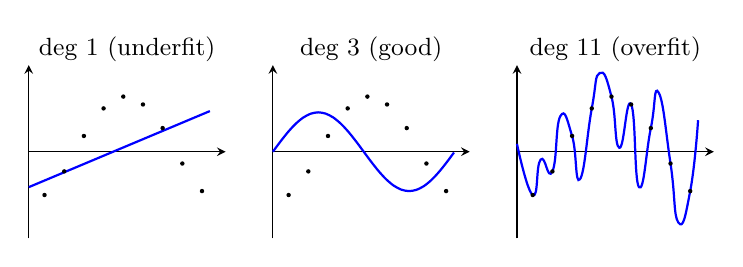
\begin{tikzpicture}[scale=0.5,>=stealth]
% three panels: deg1 underfit / deg3 good / deg11 overfit
\begin{scope}
\draw[->] (0,0)--(5,0); \draw[->] (0,-2.2)--(0,2.2);
\node at (2.5,2.6) {\small deg 1 (underfit)};
\draw[blue,thick,domain=0:4.6] plot (\x,{-0.9+0.42*\x});
\foreach \p in {(0.4,-1.1),(0.9,-0.5),(1.4,0.4),(1.9,1.1),(2.4,1.4),(2.9,1.2),(3.4,0.6),(3.9,-0.3),(4.4,-1.0)} \fill \p circle (1.6pt);
\end{scope}
\begin{scope}[xshift=6.2cm]
\draw[->] (0,0)--(5,0); \draw[->] (0,-2.2)--(0,2.2);
\node at (2.5,2.6) {\small deg 3 (good)};
\draw[blue,thick,domain=0:4.6,smooth] plot (\x,{sin(\x*78)});
\foreach \p in {(0.4,-1.1),(0.9,-0.5),(1.4,0.4),(1.9,1.1),(2.4,1.4),(2.9,1.2),(3.4,0.6),(3.9,-0.3),(4.4,-1.0)} \fill \p circle (1.6pt);
\end{scope}
\begin{scope}[xshift=12.4cm]
\draw[->] (0,0)--(5,0); \draw[->] (0,-2.2)--(0,2.2);
\node at (2.5,2.6) {\small deg 11 (overfit)};
\draw[blue,thick,domain=0:4.6,smooth,tension=0.9]
 plot coordinates {(0,0.2)(0.4,-1.1)(0.6,-0.2)(0.9,-0.5)(1.1,0.9)(1.4,0.4)(1.6,-0.7)(1.9,1.1)(2.1,2.0)(2.4,1.4)(2.6,0.1)(2.9,1.2)(3.1,-0.9)(3.4,0.6)(3.6,1.5)(3.9,-0.3)(4.1,-1.8)(4.4,-1.0)(4.6,0.8)};
\foreach \p in {(0.4,-1.1),(0.9,-0.5),(1.4,0.4),(1.9,1.1),(2.4,1.4),(2.9,1.2),(3.4,0.6),(3.9,-0.3),(4.4,-1.0)} \fill \p circle (1.6pt);
\end{scope}
\end{tikzpicture}

\caption{Same data, three feature maps. Notice the degree-1 panel misses
the pattern (underfit), degree-3 captures it, degree-11 threads every
noise point (overfit) --- minimum training error is NOT the goal.
Regenerate: \ttfamily figures/ch08\_overfit\_panel.tex.}
\label{fig:overfit}
\end{figure}

\begin{lstlisting}[caption={\ttfamily code/ch08\_poly\_overfit.py --- fit
degree $d$, report training RSS vs.\ error against the true function.}]
import numpy as np
np.set_printoptions(precision=4, suppress=True)

rng = np.random.default_rng(1)
x = np.sort(rng.uniform(0, 1, 12))
y = np.sin(2 * np.pi * x) + 0.15 * rng.standard_normal(12)

def fit_eval(deg):
    A = np.vander(x, deg + 1, increasing=True)
    c, res, *_ = np.linalg.lstsq(A, y, rcond=None)
    rss_train = ((y - A @ c)**2).sum()
    xg = np.linspace(0, 1, 400)
    yg = np.sin(2 * np.pi * xg)
    rss_true = ((yg - np.vander(xg, deg + 1, increasing=True) @ c)**2).mean()
    return rss_train, rss_true

print("deg  train-RSS   true-RMS-error")
for d in [1, 3, 5, 11]:
    tr, te = fit_eval(d)
    print(f"{d:2d}   {tr:8.4f}   {te:9.4f}")
\end{lstlisting}

\begin{lstlisting}[caption={Output of the overfit demo. Notice training
RSS decreases monotonically to zero --- projections only get closer ---
while the true error turns around and explodes at degree 11, where $A$
has a column per data point.}]
deg  train-RSS   true-RMS-error
 1     2.4333      0.2277
 3     0.0628      0.0099
 5     0.0279      0.0054
11     0.0000   25288.1886
\end{lstlisting}

\begin{exercise}[hard]
Explain why train-RSS is monotone non-increasing in the number of columns
of $A$ --- a one-line argument from projection geometry --- and why the
argument says nothing about unseen data.
\begin{solution}
Adding a column enlarges $\operatorname{col}(A)$ to a bigger subspace, so
the closest point can only get closer: projection distance is monotone in
subspace inclusion. Unseen data isn't in the space we minimized over ---
the minimizer just moved $\mathbf b$'s projection, not the world's.
\end{solution}
\end{exercise}

\section{Solving in practice: QR, not \texorpdfstring{$A^{T}A$}{A^TA}}\label{sec:lstsq-qr}

The normal equations are the right \emph{theorem} and the wrong
\emph{algorithm}. $A^{T}A$ squares the condition number
--- $\kappa(A^{T}A)=\kappa(A)^{2}$ --- so solving it throws away half the
digits before arithmetic even starts. Chapter 5's QR factorization dodges
it: with $A=QR$,
\[
A^{T}A\hat{\mathbf x}=A^{T}\mathbf b
\iff R\hat{\mathbf x}=Q^{T}\mathbf b ,
\]
a triangular solve that never forms $A^{T}A$. When $A$ has full column
rank, $R$ is invertible and $\hat{\mathbf x}$ is \emph{unique}
(its uniqueness is a [hard] exercise below).

\begin{example}[Same fit, stable route]\label{ex:qrsolve}
\textbf{Strategy.} Build a pathological $A$: features $1,x,x^{2}$ sampled
on a window only $10^{-3}$ wide, so the columns are nearly parallel. Fit
the same noise-free quadratic both ways and compare against truth.

\textbf{Solution.} $\kappa(A)\approx5\times10^{7}$, so
$\kappa(A^{T}A)\approx3\times10^{15}$ --- one digit short of float64's
entire budget. The listing shows the consequence exactly: the $A^{T}A$
solve lands 0.74 from truth while \texttt{np.linalg.lstsq} (QR/SVD
internals) recovers the coefficients to $10^{-9}$.
\end{example}

\begin{lstlisting}[caption={\ttfamily code/ch08\_ata\_vs\_lstsq.py ---
same problem, two routes; the condition square is visible in the answer.}]
import numpy as np
np.set_printoptions(precision=6, suppress=True)

# x and x^2 over a window 1e-3 wide: the columns are nearly parallel
rng = np.random.default_rng(0)
n = 200
x = 1 + 0.001 * rng.random(n)
y = 2 - 3 * x + 0.5 * x**2            # exact quadratic data, no noise
A = np.column_stack([np.ones(n), x, x**2])
print("cond(A)      = %.3e" % np.linalg.cond(A))
print("cond(A^T A)  = %.3e   <- the square" % np.linalg.cond(A.T @ A))
x_ata = np.linalg.solve(A.T @ A, A.T @ y)
x_lstsq, res, rank, sv = np.linalg.lstsq(A, y, rcond=None)
print("x via A^T A solve   :", x_ata)
print("x via np.linalg.lstsq:", x_lstsq)
print("truth               : [ 2. -3.  0.5]")
print("err A^T A : %.3e" % np.linalg.norm(x_ata - np.array([2., -3., .5])))
print("err lstsq : %.3e" % np.linalg.norm(x_lstsq - np.array([2., -3., .5])))
\end{lstlisting}

\begin{lstlisting}[caption={Output of the two-route comparison. The
computed $\kappa(A^{T}A)=3.267\times10^{15}$ is float64's own answer ---
about 14\% off the exact square $2.86\times10^{15}$, because the product
matrix is already so ill-conditioned that even its condition number
loses precision. Either way the $A^{T}A$ answer visibly differs from
truth while lstsq is exact. Same math, different arithmetic.}]
cond(A)      = 5.350e+07
cond(A^T A)  = 3.267e+15   <- the square
x via A^T A solve   : [ 2.301033 -3.601757  0.800724]
x via np.linalg.lstsq: [ 2.  -3.  0.5]
truth               : [ 2. -3.  0.5]
err A^T A : 7.370e-01
err lstsq : 2.752e-09
\end{lstlisting}

\begin{figure}[htbp]
\centering
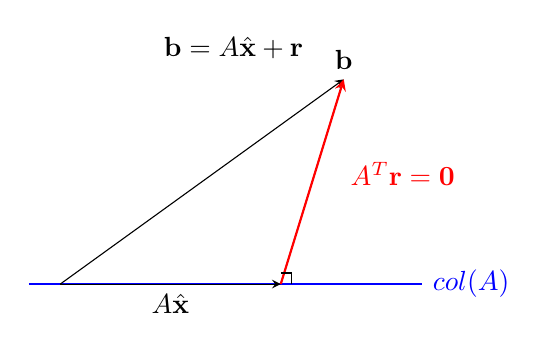
\begin{tikzpicture}[scale=1.0,>=stealth]
% col(A) as horizontal line (1-D), A xhat on it, r vertical
\draw[thick,blue] (-0.4,0) -- (4.6,0) node[right]{$\operatorname{col}(A)$};
\coordinate (O) at (0,0);
\coordinate (p) at (2.8,0);
\coordinate (b) at (3.6,2.6);
\draw[->] (O) -- (p) node[midway,below]{$A\hat{\mathbf x}$};
\draw[->] (O) -- (b) node[above]{$\mathbf b$};
\draw[->,thick,red] (p) -- (b);
\draw (2.8,0.14) -- (2.94,0.14) -- (2.94,0);
\node[red] at (4.35,1.4) {$A^{T}\mathbf r=\mathbf 0$};
\node at (2.2,3.0) {$\mathbf b=A\hat{\mathbf x}+\mathbf r$};
\end{tikzpicture}

\caption{The normal equations geometrically. Notice $A^{T}\mathbf r=
\mathbf0$ is one sentence --- ``the leftover is perpendicular to
everything $A$ can reach'' --- and it pins $\hat{\mathbf x}$ uniquely
when the columns are independent. Regenerate:
\ttfamily figures/ch08\_normal\_geometry.tex.}
\label{fig:normal-geo}
\end{figure}

\begin{exercise}[medium]
A feature is measured in millimeters instead of meters (same data, column
$\times1000$). What happens to $\kappa(A)$ and to the fitted
\emph{predictions}?
\begin{solution}
$\kappa(A)$ grows (column scales diverge --- the condition number sees the
ratio). Predictions are unchanged: $\operatorname{col}(A)$ is the same
subspace, so the projection is the same; only the coefficient units move.
This is why scaling helps conditioning but cannot change the fit.
\end{solution}
\end{exercise}

\section{Residuals, \texorpdfstring{$R^{2}$}{R2}, and honest evaluation}\label{sec:lstsq-eval}

\begin{definition}[Residuals and $R^{2}$]\index{residual}\index{R-squared@$R^2$}
The residual $\mathbf r=\mathbf b-A\hat{\mathbf x}$ is what's left over.
With $\bar y$ the mean of $\mathbf b$,
\[
R^{2}=1-\frac{\lVert\mathbf r\rVert^{2}}{\lVert\mathbf b-\bar y\,\mathbf1\rVert^{2}}
\]
is the fraction of variance the fit explains --- $1$ is perfect, $0$ is no
better than predicting the mean, negative means \emph{worse} than the
mean.
\end{definition}

\begin{example}[Reading a residual plot]\label{ex:resplot}
\textbf{Strategy.} A good fit leaves structureless residue: the model
already ate the pattern. Plot $r_i$ against $\hat y_i$ (or $x_i$) and ask
what's left.

\textbf{Solution.} Figure~\ref{fig:residplot}: left panel is random
scatter about zero --- done. Right panel curves systematically --- the
model missed a feature (here a quadratic term); more data of the same
kind won't help, a better $\operatorname{col}(A)$ will.
\end{example}

\begin{figure}[htbp]
\centering
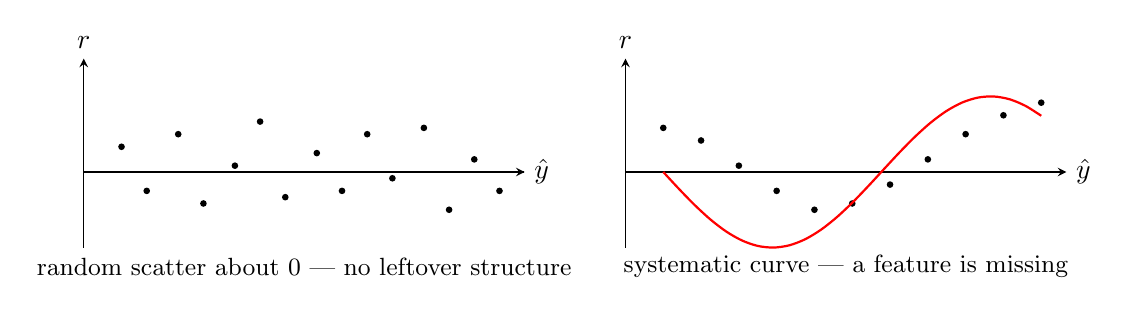
\begin{tikzpicture}[scale=0.8,>=stealth]
% residual vs fitted: random scatter = good; funnel/fan = model missing structure
\draw[->] (0,-1.6) -- (7,-1.6) node[right]{$\hat y$};
\draw[->] (0,-2.8) -- (0,0.2) node[above]{$r$};
\draw[dashed] (0,-1.6) -- (7,-1.6);
\foreach \p in {(0.6,-1.2),(1.0,-1.9),(1.5,-1.0),(1.9,-2.1),(2.4,-1.5),(2.8,-0.8),(3.2,-2.0),(3.7,-1.3),(4.1,-1.9),(4.5,-1.0),(4.9,-1.7),(5.4,-0.9),(5.8,-2.2),(6.2,-1.4),(6.6,-1.9)} \fill \p circle (1.5pt);
\node at (3.5,-3.1) {\small random scatter about 0 --- no leftover structure};
% right panel: curved pattern (bad)
\begin{scope}[xshift=8.6cm]
\draw[->] (0,-1.6) -- (7,-1.6) node[right]{$\hat y$};
\draw[->] (0,-2.8) -- (0,0.2) node[above]{$r$};
\foreach \p in {(0.6,-0.9),(1.2,-1.1),(1.8,-1.5),(2.4,-1.9),(3.0,-2.2),(3.6,-2.1),(4.2,-1.8),(4.8,-1.4),(5.4,-1.0),(6.0,-0.7),(6.6,-0.5)} \fill \p circle (1.5pt);
\draw[red,thick,domain=0.6:6.6,smooth] plot (\x,{-1.6-1.2*sin((\x-0.6)*52)});
\node at (3.5,-3.1) {\small systematic curve --- a feature is missing};
\end{scope}
\end{tikzpicture}

\caption{Residual diagnostics. Notice the left panel is scatter with no
pattern (nothing left to learn) while the right panel's systematic curve
means the feature map is missing something --- the fix is a better basis,
not more rows. Regenerate: \ttfamily figures/ch08\_residual\_plot.tex.}
\label{fig:residplot}
\end{figure}

Two disciplines protect honesty:

\begin{itemize}
\item \textbf{Train/test split.} Evaluating on the same rows that produced
$\hat{\mathbf x}$ rewards memorization (Figure~\ref{fig:overfit}).
Hold back a test split --- Figure~\ref{fig:traintest} --- and score there;
it is the only measurement that means anything.
\item \textbf{$R^{2}$ is not causality.} $R^{2}\approx0.99$ says the
features predict the target \emph{in this sample}. Nothing in the
projection knows why the columns correlate --- a $0.99$ fit between ice
cream and drowning is real arithmetic and fake science.
\end{itemize}

\begin{figure}[htbp]
\centering
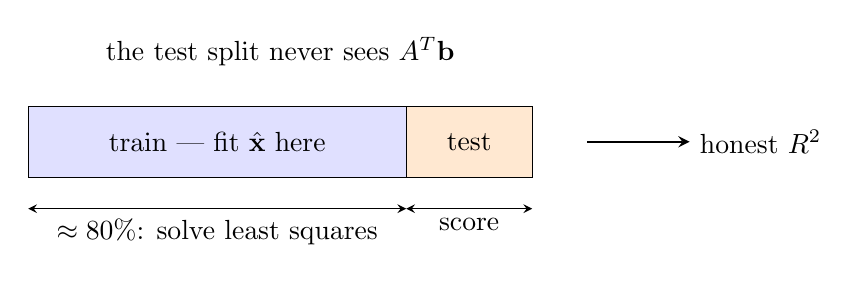
\begin{tikzpicture}[scale=1.0,>=stealth]
% dataset bar split: train (fit) | test (score)
\draw[fill=blue!12] (0,0) rectangle (4.8,0.9);
\draw[fill=orange!18] (4.8,0) rectangle (6.4,0.9);
\node at (2.4,0.45) {train --- fit $\hat{\mathbf x}$ here};
\node at (5.6,0.45) {test};
\draw[<->] (0,-0.4) -- (4.8,-0.4) node[midway,below]{$\approx80\%$: solve least squares};
\draw[<->] (4.8,-0.4) -- (6.4,-0.4) node[midway,below]{score};
\draw[->,thick] (7.1,0.45) -- (8.4,0.45) node[right]{honest $R^2$};
\node[align=left] at (3.2,1.6) {the test split never sees $A^T\mathbf b$};
\end{tikzpicture}

\caption{The honest protocol. Notice the test split contributes nothing
to $A^{T}A\hat{\mathbf x}=A^{T}\mathbf b$ --- it exists only to be scored.
Regenerate: \ttfamily figures/ch08\_traintest.tex.}
\label{fig:traintest}
\end{figure}

\begin{example}[Capstone: our own LinearRegression vs.\ sklearn]\label{ex:capstone}
\textbf{Strategy.} Implement \texttt{fit} as the QR route of
Section~\ref{sec:lstsq-qr} (with the intercept column handled inside),
\texttt{predict} as $A\hat{\mathbf x}$, and \texttt{r2} by definition.
Compare against \texttt{sklearn.linear\_model.LinearRegression} on a
300-row synthetic housing set.

\textbf{Solution.} The listing shows our coefficients matching sklearn's
to $4\times10^{-14}$ --- the library is doing exactly this math, nothing
more. $R^{2}=0.987$ both ways.
\end{example}

\begin{lstlisting}[caption={\ttfamily code/ch08\_capstone\_linreg.py ---
\texttt{mlscratch} vs.\ \texttt{sklearn}: the whole ``library algorithm''
is the QR solve of this chapter.}]
import numpy as np
from sklearn.linear_model import LinearRegression
np.set_printoptions(precision=4, suppress=True)

# mlscratch: our own least-squares fitter, QR route from ch.5
class LinearRegression_scratch:
    def fit(self, A, y):
        A1 = np.column_stack([np.ones(len(A)), A])  # intercept column!
        Q, R = np.linalg.qr(A1)
        self.coef_ = np.linalg.solve(R, Q.T @ y)
        self.intercept_, self.slopes_ = self.coef_[0], self.coef_[1:]
        return self
    def predict(self, A):
        return self.intercept_ + A @ self.slopes_
    def r2(self, A, y):
        r = y - self.predict(A)
        return 1 - (r @ r) / ((y - y.mean()) @ (y - y.mean()))

# real-ish dataset: floor area, rooms, age -> apartment price
rng = np.random.default_rng(2)
n = 300
area = rng.uniform(30, 120, n)
rooms = rng.integers(1, 5, n).astype(float)
age = rng.uniform(0, 40, n)
price = 8 + 2.1 * area + 4 * rooms - 0.15 * age + 6 * rng.standard_normal(n)
X = np.column_stack([area, rooms, age])

ours = LinearRegression_scratch().fit(X, price)
ref = LinearRegression().fit(X, price)
print("ours   intercept %.4f  slopes %s" % (ours.intercept_, ours.slopes_))
print("sklearn intercept %.4f  slopes %s" % (ref.intercept_, ref.coef_))
print("max |coef diff| = %.2e" % np.abs(ours.coef_ - np.append(ref.intercept_, ref.coef_)).max())
print("R^2 ours   = %.4f" % ours.r2(X, price))
print("R^2 sklearn= %.4f" % ref.score(X, price))
\end{lstlisting}

\begin{lstlisting}[caption={Output of the capstone. Notice the
coefficients agree to machine precision --- least squares via QR IS what
the library computes, and your implementation is the real thing, not a
toy.}]
ours   intercept 8.2343  slopes [ 2.0965  4.1166 -0.1587]
sklearn intercept 8.2343  slopes [ 2.0965  4.1166 -0.1587]
max |coef diff| = 4.26e-14
R^2 ours   = 0.9874
R^2 sklearn= 0.9874
\end{lstlisting}

\begin{exercise}[easy]
A model has $R^{2}=0.4$ on train and $0.38$ on test. A second has
$R^{2}=0.97$ train, $0.55$ test. Which is better and why?
\begin{solution}
The second memorized: its train score proves the columns could fit noise.
The first generalizes --- its test score is the honest number; prefer it
unless the gap in accuracy itself is disqualifying.
\end{solution}
\end{exercise}

\begin{exercise}[hard --- derive]
Weighted least squares: minimize
$\lVert W(\mathbf b-A\mathbf x)\rVert^{2}$ with $W$ diagonal and positive.
Derive the weighted normal equations
$A^{T}W^{2}A\hat{\mathbf x}=A^{T}W^{2}\mathbf b$, and say what the weights
mean physically.
\begin{solution}
It's ordinary least squares on the row-scaled system
$A'=WA$, $\mathbf b'=W\mathbf b$: orthogonal residual
$A'^{T}(\mathbf b'-A'\hat{\mathbf x})=\mathbf0$ expands to
$A^{T}W^{2}(\mathbf b-A\hat{\mathbf x})=\mathbf0$.
Weight $w_{ii}$ large $\Rightarrow$ row $i$ must be fit tightly ---
trusted measurements get loud votes.
\end{solution}
\end{exercise}

\section{Hand derivation}\label{sec:handderiv8}

Derive $A^{T}A\hat{\mathbf x}=A^{T}\mathbf b$ from
residual-orthogonality. Among all $\mathbf x$, the vector
$A\mathbf x$ ranges over $\operatorname{col}(A)$; the closest point of a
subspace to $\mathbf b$ is the projection $\mathbf p$ satisfying
$\mathbf b-\mathbf p\perp$ every vector in the subspace. Write
$\mathbf p=A\hat{\mathbf x}$. Perpendicularity to every column is a row
per column:
\[
A^{T}(\mathbf b-A\hat{\mathbf x})=\mathbf0
\iff A^{T}\mathbf b-A^{T}A\hat{\mathbf x}=\mathbf0
\iff A^{T}A\hat{\mathbf x}=A^{T}\mathbf b .
\]
When $A$ has full column rank, $A^{T}A$ is positive definite
($\mathbf x^{T}A^{T}A\mathbf x=\lVert A\mathbf x\rVert^{2}>0$ for
$\mathbf x\ne\mathbf0$), hence invertible, hence the solution unique.
(Calculus route --- gradient of $\lVert\mathbf b-A\mathbf x\rVert^{2}$ ---
lands here too; it waits for chapter 14.)

\section{Common mistakes}\label{sec:lsq-mistakes}

\begin{tripwire}[{Forgetting the intercept column}]
Without $\mathbf 1$ in $A$ the model must pass through the origin ---
every prediction carries a systematic offset. Always
\texttt{column\_stack([ones, ...])}.
\end{tripwire}

\begin{tripwire}[{Forming $A^{T}A$ when QR is cheaper and stabler}]
$\kappa(A^{T}A)=\kappa(A)^{2}$: near-parallel columns turn a hard problem
into an impossible one, as the demo showed (err $0.74$ vs $10^{-9}$ on
the same data). Solve $R\hat{\mathbf x}=Q^{T}\mathbf b$, or call
\texttt{np.linalg.lstsq} and let LAPACK choose.
\end{tripwire}

\begin{tripwire}[{Letting unscaled features wreck conditioning}]
A column in millimeters beside one in kilometers gives $10^{6}$ scale
ratios for free. Center and scale features first --- it fixes $\kappa(A)$
without changing $\operatorname{col}(A)$.
\end{tripwire}

\begin{tripwire}[{Evaluating on training data and calling it performance}]
Train-RSS is monotone in columns and reaches zero exactly when $A$ can
memorize. A model that aces its own exam learned nothing. The test split
is the only number that counts.
\end{tripwire}

\begin{tripwire}[{Reading $R^{2}$ as a certificate of causality}]
$R^{2}$ measures in-sample correlation structure, nothing else. A high
$R^{2}$ between an umbrella index and rain is prediction; believing
umbrellas cause rain is a different discipline entirely.
\end{tripwire}

\section{Summary}

\begin{center}
\begin{tabularx}{\textwidth}{l>{\raggedright\arraybackslash}X}
\toprule
\textbf{Object} & \textbf{What you need to know}\\
\midrule
Least squares & minimize $\lVert\mathbf b-A\mathbf x\rVert^2$; the best
fit is the projection of $\mathbf b$ on $\operatorname{col}(A)$ \\
Normal equations & $A^{T}A\hat{\mathbf x}=A^{T}\mathbf b$, from
$A^{T}\mathbf r=\mathbf0$; unique iff full column rank \\
Design matrix & one column per feature + the intercept column of ones;
``linear'' $=$ linear in coefficients \\
Feature maps & $[\mathbf1\ \mathbf x\ \mathbf x^2\ \dots]$ lets the same
machinery fit curves; more columns $\Rightarrow$ less train RSS \\
Compute route & QR: $R\hat{\mathbf x}=Q^{T}\mathbf b$; forming $A^{T}A$
squares $\kappa$ \\
Residuals & good fit $\Rightarrow$ structureless scatter; patterns mean a
missing feature \\
$R^{2}$ & $1-\mathrm{RSS}/\mathrm{TSS}$; measures correlation in-sample,
never causality \\
Evaluation & train/test split: the test rows must not touch
$A^{T}\mathbf b$ \\
\bottomrule
\end{tabularx}
\end{center}

\section*{Additional exercises}
\addcontentsline{toc}{section}{Additional exercises}

\begin{exercise}[easy]
Write the design matrix for fitting $y=a+bx_1+cx_2$ to
$(x_1,x_2,y)\in\{(0,0,1),(1,0,3),(0,1,2),(1,1,5)\}$ and state the normal
equations.
\end{exercise}

\begin{exercise}[easy]
Given $\hat{\mathbf x}=(1.0,0.9)$ for Example~\ref{ex:linefit}, predict
$y$ at $x=5$ and at $x=0.5$. Which prediction do you trust more and why?
\end{exercise}

\begin{exercise}[easy]
If $\mathbf b\in\operatorname{col}(A)$ already, what is the least-squares
residual? What is $R^{2}$?
\end{exercise}

\begin{exercise}[easy]
Compute $R^{2}$ for the fit of Example~\ref{ex:linefit} (RSS $=0.7$,
$\mathbf b$'s mean $3.25$, TSS $=5.75$).
\end{exercise}

\begin{exercise}[medium]
Show the projection $P=A(A^{T}A)^{-1}A^{T}$ applied to $\mathbf b$ gives
exactly $A\hat{\mathbf x}$, and verify $P^2=P$.
\end{exercise}

\begin{exercise}[medium]
For the four points of Example~\ref{ex:linefit}, add the point
$(5,10)$ and refit. Which coefficient moves more, and what does that say
about leverage?
\end{exercise}

\begin{exercise}[medium]
In code: take the capstone dataset, drop the intercept column, refit, and
report what happens to $R^{2}$ and the residual mean.
\end{exercise}

\begin{exercise}[medium]
Show $\lVert\mathbf b\rVert^{2}=\lVert A\hat{\mathbf x}\rVert^{2}
+\lVert\mathbf r\rVert^{2}$ (Pythagoras for least squares) and connect it
to $R^{2}$.
\end{exercise}

\begin{exercise}[medium]
A dataset has 8 points lying exactly on a cubic. Fit degrees
1--6 in code and plot train RSS vs.\ degree --- where does the elbow sit
and why?
\end{exercise}

\begin{exercise}[hard]
Prove the least-squares minimizer is unique iff $A$ has full column rank
(show both directions: $\ker A$ nontrivial $\Rightarrow$ a family of
minimizers; trivial $\Rightarrow$ $A^{T}A$ positive definite).
\end{exercise}

\begin{exercise}[hard]
Generalized least squares: minimize
$\lVert\mathbf b-A\mathbf x\rVert_{C}^{2}=(\mathbf b-A\mathbf x)^{T}C^{-1}
(\mathbf b-A\mathbf x)$ for covariance $C\succ0$. Derive the analog of the
normal equations and interpret $C=I$ and $C$ diagonal.
\end{exercise}

\begin{exercise}[hard]
Show that $R^{2}$ computed on the training set equals the squared
correlation between $\mathbf b$ and $A\hat{\mathbf x}$ when an intercept
is present --- and give a counterexample when it is not.
\end{exercise}

\begin{exercise}[hard]
Implement leave-one-out cross-validation for the capstone data in code:
fit on $n-1$ rows, score the held-out row, average. Compare LOO $R^{2}$
to train $R^{2}$ and explain any gap in the language of this chapter.
\end{exercise}

\section*{Notes}
\addcontentsline{toc}{section}{Notes}

\chapternotes{%
Least squares as the application spine follows VMLS part III \cite{vmls}
--- including the ``linear in coefficients'' framing and the
train/test honesty rules; the projection derivation is Strang's 18.06SC
Unit II \cite{ocw1806sc} and \cite{ila} ch.~5; the conditioning warning
and residual diagnostics follow MML ch.~9 \cite{mml}. The calculus proof
is deferred to ch.~14 where gradients are in scope.}
